% !TeX root = ../el-proceso-de-software.tex


\begin{enunciado}
    Modifica el tablero que se muestra en la \autoref{fig:el_proceso_ej1_kanban} para para que sea un tablero Kanban.
\end{enunciado}

\begin{figure}[h!]
    \centering
    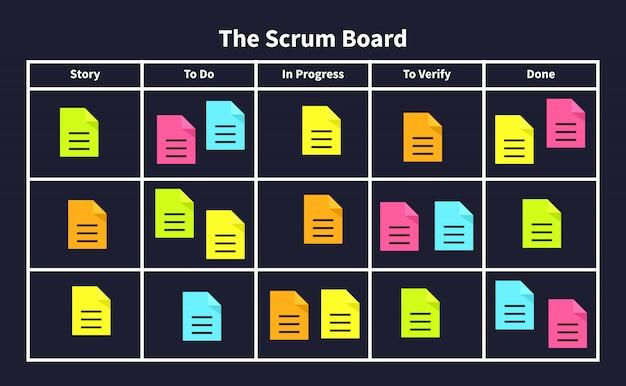
\includegraphics[width=0.75\textwidth]{../rsc/el_proceso_ej1_scrum}
    \caption{Tablero scrum para el ejercicio 1}
    \label{fig:el_proceso_ej1_kanban}
\end{figure}

\begin{solucion}
    Para transformar el tablero Scrum en un tablero Kanban, se deben seguir los siguientes pasos:
    \begin{itemize}
        \item Renombrar las columnas de \textquote{In progress} y \textquote{Verify} a \textquote{Development} y \textquote{Testing} y, dividirlas en \textquote{En proceso} y \textquote{realizadas}.
        \item Añadir una columna de \textquote{Backlog} para las tareas pendientes.
        \item Añadir una columna de \textquote{Deployment} para las tareas que ya están listas para ser desplegadas.
    \end{itemize}
\end{solucion}